% chapter1.tex
\section{Basic Concepts of Probability}

Probability is a measure of the confidence that an event will occur.

\subsection{Sample Space}
Defined as the set of all possible outcomes of an experiment:
\[
\Omega = \{ \omega_1, \omega_2, ..., \omega_n \}
\]

\subsection{Classical Probability}
If all events are equally likely:
\[
P(A) = \frac{|A|}{|\Omega|}
\]

\subsection{Example}
Consider a random coin toss, where \( \Omega = \{ \text{Heads}, \text{Tails} \} \).
The probability of getting heads:
\[
P(\text{Heads}) = \frac{1}{2}
\]

\begin{figure}[h]
    \centering
    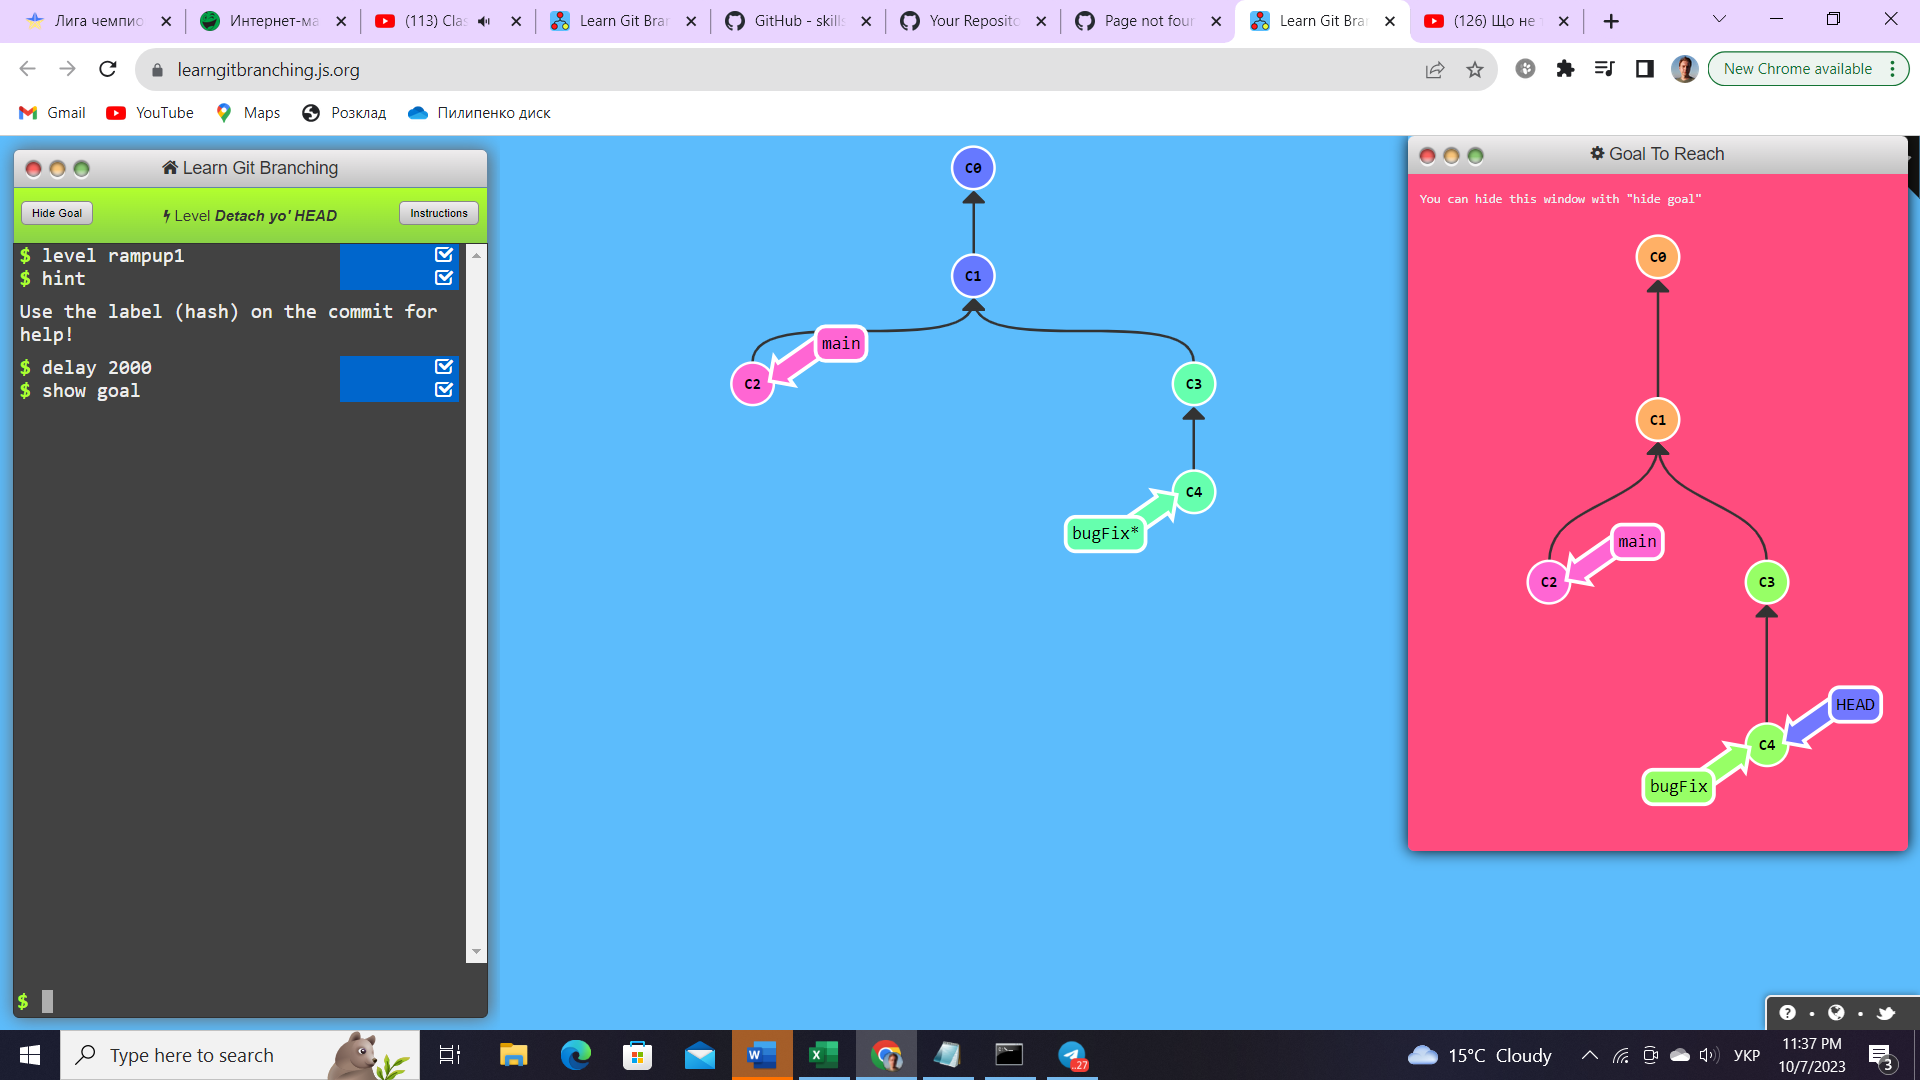
\includegraphics[width=0.7\textwidth]{images/example.png}
    \caption{Graphical representation of probability}
\end{figure}